\documentclass[12pt]{article}
\usepackage[canadien]{babel} 
\usepackage[utf8]{inputenc}
\usepackage[T1]{fontenc}
\usepackage{fancyhdr}
\usepackage{graphicx}
\usepackage{enumerate}
%\usepackage{enumitem}
\usepackage{amsmath}
\usepackage{amssymb}
\usepackage{subfigure}
\usepackage{amsmath}
\usepackage{amssymb}
\usepackage{bm}
\usepackage{url}
\usepackage{todonotes}

% If your paper is accepted, change the options for the package
% aistats2e as follows:
%
%\usepackage[accepted]{aistats2e}
%
% This option will print headings for the title of your paper and
% headings for the authors names, plus a copyright note at the end of
% the first column of the first page.
\setlength{\parindent}{0cm}
\addtolength{\oddsidemargin}{-2cm}
\addtolength{\evensidemargin}{-2cm}
\setlength{\textwidth}{17.78cm}
\addtolength{\topmargin}{-2.25cm}
\setlength{\textheight}{24.24cm}
\addtolength{\parskip}{5mm}
\pagestyle{fancy}

%************
%* COMMANDS *
%************

%%%%% NEW MATH DEFINITIONS %%%%%

% Mark sections of captions for referring to divisions of figures
\newcommand{\figleft}{{\em (Left)}}
\newcommand{\figcenter}{{\em (Center)}}
\newcommand{\figright}{{\em (Right)}}
\newcommand{\figtop}{{\em (Top)}}
\newcommand{\figbottom}{{\em (Bottom)}}
\newcommand{\captiona}{{\em (a)}}
\newcommand{\captionb}{{\em (b)}}
\newcommand{\captionc}{{\em (c)}}
\newcommand{\captiond}{{\em (d)}}

% Highlight a newly defined term
\newcommand{\newterm}[1]{{\bf #1}}


% Figure reference, lower-case.
\def\figref#1{figure~\ref{#1}}
% Figure reference, capital. For start of sentence
\def\Figref#1{Figure~\ref{#1}}
\def\twofigref#1#2{figures \ref{#1} and \ref{#2}}
\def\quadfigref#1#2#3#4{figures \ref{#1}, \ref{#2}, \ref{#3} and \ref{#4}}
% Section reference, lower-case.
\def\secref#1{section~\ref{#1}}
% Section reference, capital.
\def\Secref#1{Section~\ref{#1}}
% Reference to two sections.
\def\twosecrefs#1#2{sections \ref{#1} and \ref{#2}}
% Reference to three sections.
\def\secrefs#1#2#3{sections \ref{#1}, \ref{#2} and \ref{#3}}
% Reference to an equation, lower-case.
\def\eqref#1{equation~\ref{#1}}
% Reference to an equation, upper case
\def\Eqref#1{Equation~\ref{#1}}
% A raw reference to an equation---avoid using if possible
\def\plaineqref#1{\ref{#1}}
% Reference to a chapter, lower-case.
\def\chapref#1{chapter~\ref{#1}}
% Reference to an equation, upper case.
\def\Chapref#1{Chapter~\ref{#1}}
% Reference to a range of chapters
\def\rangechapref#1#2{chapters\ref{#1}--\ref{#2}}
% Reference to an algorithm, lower-case.
\def\algref#1{algorithm~\ref{#1}}
% Reference to an algorithm, upper case.
\def\Algref#1{Algorithm~\ref{#1}}
\def\twoalgref#1#2{algorithms \ref{#1} and \ref{#2}}
\def\Twoalgref#1#2{Algorithms \ref{#1} and \ref{#2}}
% Reference to a part, lower case
\def\partref#1{part~\ref{#1}}
% Reference to a part, upper case
\def\Partref#1{Part~\ref{#1}}
\def\twopartref#1#2{parts \ref{#1} and \ref{#2}}

\def\ceil#1{\lceil #1 \rceil}
\def\floor#1{\lfloor #1 \rfloor}
\def\1{\bm{1}}
\newcommand{\train}{\mathcal{D}}
\newcommand{\valid}{\mathcal{D_{\mathrm{valid}}}}
\newcommand{\test}{\mathcal{D_{\mathrm{test}}}}

\def\eps{{\epsilon}}


% Random variables
\def\reta{{\textnormal{$\eta$}}}
\def\ra{{\textnormal{a}}}
\def\rb{{\textnormal{b}}}
\def\rc{{\textnormal{c}}}
\def\rd{{\textnormal{d}}}
\def\re{{\textnormal{e}}}
\def\rf{{\textnormal{f}}}
\def\rg{{\textnormal{g}}}
\def\rh{{\textnormal{h}}}
\def\ri{{\textnormal{i}}}
\def\rj{{\textnormal{j}}}
\def\rk{{\textnormal{k}}}
\def\rl{{\textnormal{l}}}
% rm is already a command, just don't name any random variables m
\def\rn{{\textnormal{n}}}
\def\ro{{\textnormal{o}}}
\def\rp{{\textnormal{p}}}
\def\rq{{\textnormal{q}}}
\def\rr{{\textnormal{r}}}
\def\rs{{\textnormal{s}}}
\def\rt{{\textnormal{t}}}
\def\ru{{\textnormal{u}}}
\def\rv{{\textnormal{v}}}
\def\rw{{\textnormal{w}}}
\def\rx{{\textnormal{x}}}
\def\ry{{\textnormal{y}}}
\def\rz{{\textnormal{z}}}

% Random vectors
\def\rvepsilon{{\mathbf{\epsilon}}}
\def\rvtheta{{\mathbf{\theta}}}
\def\rva{{\mathbf{a}}}
\def\rvb{{\mathbf{b}}}
\def\rvc{{\mathbf{c}}}
\def\rvd{{\mathbf{d}}}
\def\rve{{\mathbf{e}}}
\def\rvf{{\mathbf{f}}}
\def\rvg{{\mathbf{g}}}
\def\rvh{{\mathbf{h}}}
\def\rvu{{\mathbf{i}}}
\def\rvj{{\mathbf{j}}}
\def\rvk{{\mathbf{k}}}
\def\rvl{{\mathbf{l}}}
\def\rvm{{\mathbf{m}}}
\def\rvn{{\mathbf{n}}}
\def\rvo{{\mathbf{o}}}
\def\rvp{{\mathbf{p}}}
\def\rvq{{\mathbf{q}}}
\def\rvr{{\mathbf{r}}}
\def\rvs{{\mathbf{s}}}
\def\rvt{{\mathbf{t}}}
\def\rvu{{\mathbf{u}}}
\def\rvv{{\mathbf{v}}}
\def\rvw{{\mathbf{w}}}
\def\rvx{{\mathbf{x}}}
\def\rvy{{\mathbf{y}}}
\def\rvz{{\mathbf{z}}}

% Elements of random vectors
\def\erva{{\textnormal{a}}}
\def\ervb{{\textnormal{b}}}
\def\ervc{{\textnormal{c}}}
\def\ervd{{\textnormal{d}}}
\def\erve{{\textnormal{e}}}
\def\ervf{{\textnormal{f}}}
\def\ervg{{\textnormal{g}}}
\def\ervh{{\textnormal{h}}}
\def\ervi{{\textnormal{i}}}
\def\ervj{{\textnormal{j}}}
\def\ervk{{\textnormal{k}}}
\def\ervl{{\textnormal{l}}}
\def\ervm{{\textnormal{m}}}
\def\ervn{{\textnormal{n}}}
\def\ervo{{\textnormal{o}}}
\def\ervp{{\textnormal{p}}}
\def\ervq{{\textnormal{q}}}
\def\ervr{{\textnormal{r}}}
\def\ervs{{\textnormal{s}}}
\def\ervt{{\textnormal{t}}}
\def\ervu{{\textnormal{u}}}
\def\ervv{{\textnormal{v}}}
\def\ervw{{\textnormal{w}}}
\def\ervx{{\textnormal{x}}}
\def\ervy{{\textnormal{y}}}
\def\ervz{{\textnormal{z}}}

% Random matrices
\def\rmA{{\mathbf{A}}}
\def\rmB{{\mathbf{B}}}
\def\rmC{{\mathbf{C}}}
\def\rmD{{\mathbf{D}}}
\def\rmE{{\mathbf{E}}}
\def\rmF{{\mathbf{F}}}
\def\rmG{{\mathbf{G}}}
\def\rmH{{\mathbf{H}}}
\def\rmI{{\mathbf{I}}}
\def\rmJ{{\mathbf{J}}}
\def\rmK{{\mathbf{K}}}
\def\rmL{{\mathbf{L}}}
\def\rmM{{\mathbf{M}}}
\def\rmN{{\mathbf{N}}}
\def\rmO{{\mathbf{O}}}
\def\rmP{{\mathbf{P}}}
\def\rmQ{{\mathbf{Q}}}
\def\rmR{{\mathbf{R}}}
\def\rmS{{\mathbf{S}}}
\def\rmT{{\mathbf{T}}}
\def\rmU{{\mathbf{U}}}
\def\rmV{{\mathbf{V}}}
\def\rmW{{\mathbf{W}}}
\def\rmX{{\mathbf{X}}}
\def\rmY{{\mathbf{Y}}}
\def\rmZ{{\mathbf{Z}}}

% Elements of random matrices
\def\ermA{{\textnormal{A}}}
\def\ermB{{\textnormal{B}}}
\def\ermC{{\textnormal{C}}}
\def\ermD{{\textnormal{D}}}
\def\ermE{{\textnormal{E}}}
\def\ermF{{\textnormal{F}}}
\def\ermG{{\textnormal{G}}}
\def\ermH{{\textnormal{H}}}
\def\ermI{{\textnormal{I}}}
\def\ermJ{{\textnormal{J}}}
\def\ermK{{\textnormal{K}}}
\def\ermL{{\textnormal{L}}}
\def\ermM{{\textnormal{M}}}
\def\ermN{{\textnormal{N}}}
\def\ermO{{\textnormal{O}}}
\def\ermP{{\textnormal{P}}}
\def\ermQ{{\textnormal{Q}}}
\def\ermR{{\textnormal{R}}}
\def\ermS{{\textnormal{S}}}
\def\ermT{{\textnormal{T}}}
\def\ermU{{\textnormal{U}}}
\def\ermV{{\textnormal{V}}}
\def\ermW{{\textnormal{W}}}
\def\ermX{{\textnormal{X}}}
\def\ermY{{\textnormal{Y}}}
\def\ermZ{{\textnormal{Z}}}

% Vectors
\def\vzero{{\bm{0}}}
\def\vone{{\bm{1}}}
\def\vmu{{\bm{\mu}}}
\def\vtheta{{\bm{\theta}}}
\def\va{{\bm{a}}}
\def\vb{{\bm{b}}}
\def\vc{{\bm{c}}}
\def\vd{{\bm{d}}}
\def\ve{{\bm{e}}}
\def\vf{{\bm{f}}}
\def\vg{{\bm{g}}}
\def\vh{{\bm{h}}}
\def\vi{{\bm{i}}}
\def\vj{{\bm{j}}}
\def\vk{{\bm{k}}}
\def\vl{{\bm{l}}}
\def\vm{{\bm{m}}}
\def\vn{{\bm{n}}}
\def\vo{{\bm{o}}}
\def\vp{{\bm{p}}}
\def\vq{{\bm{q}}}
\def\vr{{\bm{r}}}
\def\vs{{\bm{s}}}
\def\vt{{\bm{t}}}
\def\vu{{\bm{u}}}
\def\vv{{\bm{v}}}
\def\vw{{\bm{w}}}
\def\vx{{\bm{x}}}
\def\vy{{\bm{y}}}
\def\vz{{\bm{z}}}

% Elements of vectors
\def\evalpha{{\alpha}}
\def\evbeta{{\beta}}
\def\evepsilon{{\epsilon}}
\def\evlambda{{\lambda}}
\def\evomega{{\omega}}
\def\evmu{{\mu}}
\def\evpsi{{\psi}}
\def\evsigma{{\sigma}}
\def\evtheta{{\theta}}
\def\eva{{a}}
\def\evb{{b}}
\def\evc{{c}}
\def\evd{{d}}
\def\eve{{e}}
\def\evf{{f}}
\def\evg{{g}}
\def\evh{{h}}
\def\evi{{i}}
\def\evj{{j}}
\def\evk{{k}}
\def\evl{{l}}
\def\evm{{m}}
\def\evn{{n}}
\def\evo{{o}}
\def\evp{{p}}
\def\evq{{q}}
\def\evr{{r}}
\def\evs{{s}}
\def\evt{{t}}
\def\evu{{u}}
\def\evv{{v}}
\def\evw{{w}}
\def\evx{{x}}
\def\evy{{y}}
\def\evz{{z}}

% Matrix
\def\mA{{\bm{A}}}
\def\mB{{\bm{B}}}
\def\mC{{\bm{C}}}
\def\mD{{\bm{D}}}
\def\mE{{\bm{E}}}
\def\mF{{\bm{F}}}
\def\mG{{\bm{G}}}
\def\mH{{\bm{H}}}
\def\mI{{\bm{I}}}
\def\mJ{{\bm{J}}}
\def\mK{{\bm{K}}}
\def\mL{{\bm{L}}}
\def\mM{{\bm{M}}}
\def\mN{{\bm{N}}}
\def\mO{{\bm{O}}}
\def\mP{{\bm{P}}}
\def\mQ{{\bm{Q}}}
\def\mR{{\bm{R}}}
\def\mS{{\bm{S}}}
\def\mT{{\bm{T}}}
\def\mU{{\bm{U}}}
\def\mV{{\bm{V}}}
\def\mW{{\bm{W}}}
\def\mX{{\bm{X}}}
\def\mY{{\bm{Y}}}
\def\mZ{{\bm{Z}}}
\def\mBeta{{\bm{\beta}}}
\def\mPhi{{\bm{\Phi}}}
\def\mLambda{{\bm{\Lambda}}}
\def\mSigma{{\bm{\Sigma}}}

% Tensor
\DeclareMathAlphabet{\mathsfit}{\encodingdefault}{\sfdefault}{m}{sl}
\SetMathAlphabet{\mathsfit}{bold}{\encodingdefault}{\sfdefault}{bx}{n}
\newcommand{\tens}[1]{\bm{\mathsfit{#1}}}
\def\tA{{\tens{A}}}
\def\tB{{\tens{B}}}
\def\tC{{\tens{C}}}
\def\tD{{\tens{D}}}
\def\tE{{\tens{E}}}
\def\tF{{\tens{F}}}
\def\tG{{\tens{G}}}
\def\tH{{\tens{H}}}
\def\tI{{\tens{I}}}
\def\tJ{{\tens{J}}}
\def\tK{{\tens{K}}}
\def\tL{{\tens{L}}}
\def\tM{{\tens{M}}}
\def\tN{{\tens{N}}}
\def\tO{{\tens{O}}}
\def\tP{{\tens{P}}}
\def\tQ{{\tens{Q}}}
\def\tR{{\tens{R}}}
\def\tS{{\tens{S}}}
\def\tT{{\tens{T}}}
\def\tU{{\tens{U}}}
\def\tV{{\tens{V}}}
\def\tW{{\tens{W}}}
\def\tX{{\tens{X}}}
\def\tY{{\tens{Y}}}
\def\tZ{{\tens{Z}}}


% Graph
\def\gA{{\mathcal{A}}}
\def\gB{{\mathcal{B}}}
\def\gC{{\mathcal{C}}}
\def\gD{{\mathcal{D}}}
\def\gE{{\mathcal{E}}}
\def\gF{{\mathcal{F}}}
\def\gG{{\mathcal{G}}}
\def\gH{{\mathcal{H}}}
\def\gI{{\mathcal{I}}}
\def\gJ{{\mathcal{J}}}
\def\gK{{\mathcal{K}}}
\def\gL{{\mathcal{L}}}
\def\gM{{\mathcal{M}}}
\def\gN{{\mathcal{N}}}
\def\gO{{\mathcal{O}}}
\def\gP{{\mathcal{P}}}
\def\gQ{{\mathcal{Q}}}
\def\gR{{\mathcal{R}}}
\def\gS{{\mathcal{S}}}
\def\gT{{\mathcal{T}}}
\def\gU{{\mathcal{U}}}
\def\gV{{\mathcal{V}}}
\def\gW{{\mathcal{W}}}
\def\gX{{\mathcal{X}}}
\def\gY{{\mathcal{Y}}}
\def\gZ{{\mathcal{Z}}}

% Sets
\def\sA{{\mathbb{A}}}
\def\sB{{\mathbb{B}}}
\def\sC{{\mathbb{C}}}
\def\sD{{\mathbb{D}}}
% Don't use a set called E, because this would be the same as our symbol
% for expectation.
\def\sF{{\mathbb{F}}}
\def\sG{{\mathbb{G}}}
\def\sH{{\mathbb{H}}}
\def\sI{{\mathbb{I}}}
\def\sJ{{\mathbb{J}}}
\def\sK{{\mathbb{K}}}
\def\sL{{\mathbb{L}}}
\def\sM{{\mathbb{M}}}
\def\sN{{\mathbb{N}}}
\def\sO{{\mathbb{O}}}
\def\sP{{\mathbb{P}}}
\def\sQ{{\mathbb{Q}}}
\def\sR{{\mathbb{R}}}
\def\sS{{\mathbb{S}}}
\def\sT{{\mathbb{T}}}
\def\sU{{\mathbb{U}}}
\def\sV{{\mathbb{V}}}
\def\sW{{\mathbb{W}}}
\def\sX{{\mathbb{X}}}
\def\sY{{\mathbb{Y}}}
\def\sZ{{\mathbb{Z}}}

% Entries of a matrix
\def\emLambda{{\Lambda}}
\def\emA{{A}}
\def\emB{{B}}
\def\emC{{C}}
\def\emD{{D}}
\def\emE{{E}}
\def\emF{{F}}
\def\emG{{G}}
\def\emH{{H}}
\def\emI{{I}}
\def\emJ{{J}}
\def\emK{{K}}
\def\emL{{L}}
\def\emM{{M}}
\def\emN{{N}}
\def\emO{{O}}
\def\emP{{P}}
\def\emQ{{Q}}
\def\emR{{R}}
\def\emS{{S}}
\def\emT{{T}}
\def\emU{{U}}
\def\emV{{V}}
\def\emW{{W}}
\def\emX{{X}}
\def\emY{{Y}}
\def\emZ{{Z}}
\def\emSigma{{\Sigma}}

% entries of a tensor
% Same font as tensor, without \bm wrapper
\newcommand{\etens}[1]{\mathsfit{#1}}
\def\etLambda{{\etens{\Lambda}}}
\def\etA{{\etens{A}}}
\def\etB{{\etens{B}}}
\def\etC{{\etens{C}}}
\def\etD{{\etens{D}}}
\def\etE{{\etens{E}}}
\def\etF{{\etens{F}}}
\def\etG{{\etens{G}}}
\def\etH{{\etens{H}}}
\def\etI{{\etens{I}}}
\def\etJ{{\etens{J}}}
\def\etK{{\etens{K}}}
\def\etL{{\etens{L}}}
\def\etM{{\etens{M}}}
\def\etN{{\etens{N}}}
\def\etO{{\etens{O}}}
\def\etP{{\etens{P}}}
\def\etQ{{\etens{Q}}}
\def\etR{{\etens{R}}}
\def\etS{{\etens{S}}}
\def\etT{{\etens{T}}}
\def\etU{{\etens{U}}}
\def\etV{{\etens{V}}}
\def\etW{{\etens{W}}}
\def\etX{{\etens{X}}}
\def\etY{{\etens{Y}}}
\def\etZ{{\etens{Z}}}

% The true underlying data generating distribution
\newcommand{\pdata}{p_{\rm{data}}}
% The empirical distribution defined by the training set
\newcommand{\ptrain}{\hat{p}_{\rm{data}}}
\newcommand{\Ptrain}{\hat{P}_{\rm{data}}}
% The model distribution
\newcommand{\pmodel}{p_{\rm{model}}}
\newcommand{\Pmodel}{P_{\rm{model}}}
\newcommand{\ptildemodel}{\tilde{p}_{\rm{model}}}
% Stochastic autoencoder distributions
\newcommand{\pencode}{p_{\rm{encoder}}}
\newcommand{\pdecode}{p_{\rm{decoder}}}
\newcommand{\precons}{p_{\rm{reconstruct}}}

\newcommand{\laplace}{\mathrm{Laplace}} % Laplace distribution

\newcommand{\E}{\mathbb{E}}
\newcommand{\Ls}{\mathcal{L}}
\newcommand{\R}{\mathbb{R}}
\newcommand{\emp}{\tilde{p}}
\newcommand{\lr}{\alpha}
\newcommand{\reg}{\lambda}
\newcommand{\rect}{\mathrm{rectifier}}
\newcommand{\softmax}{\mathrm{softmax}}
\newcommand{\sigmoid}{\sigma}
\newcommand{\softplus}{\zeta}
\newcommand{\KL}{D_{\mathrm{KL}}}
\newcommand{\Var}{\mathrm{Var}}
\newcommand{\standarderror}{\mathrm{SE}}
\newcommand{\Cov}{\mathrm{Cov}}
% Wolfram Mathworld says $L^2$ is for function spaces and $\ell^2$ is for vectors
% But then they seem to use $L^2$ for vectors throughout the site, and so does
% wikipedia.
\newcommand{\normlzero}{L^0}
\newcommand{\normlone}{L^1}
\newcommand{\normltwo}{L^2}
\newcommand{\normlp}{L^p}
\newcommand{\normmax}{L^\infty}

\newcommand{\parents}{Pa} % See usage in notation.tex. Chosen to match Daphne's book.

\DeclareMathOperator*{\argmax}{arg\,max}
\DeclareMathOperator*{\argmin}{arg\,min}

\DeclareMathOperator{\sign}{sign}
\DeclareMathOperator{\Tr}{Tr}
\let\ab\allowbreak


%%% new
\newcommand{\diag}{\mathop{\mathrm{diag}}\nolimits}


\newif\ifexercise
\exercisetrue
%\exercisefalse

\newif\ifsolution
%\solutiontrue
\solutionfalse

\usepackage{booktabs}
%\usepackage[chapter]{algorithm}
\usepackage{algorithmic}
% Include chapter number in algorithm number
%\renewcommand{\thealgorithm}{\arabic{chapter}.\arabic{algorithm}}

\usepackage{amsthm}
\theoremstyle{definition}
\newtheorem{exercise}{Question}%[chapter]
\newtheorem{answer}{Answer} % asterisk to remove ordering
%\newcommand{\Exercise}[1]{
%\begin{exercise}
%\ifexercise#1\fi
%\end{exercise}
%}

\newcommand{\Exercise}[1]{
\ifexercise#1\fi
}

\newcommand{\Answer}[1]{
\ifsolution\begin{answer}#1\end{answer}\fi
}

\newif\ifexercise
\exercisetrue
%\exercisefalse

\newif\ifsolution
\solutiontrue
%\solutionfalse

\usepackage{enumitem}
\newcommand{\staritem}{
\addtocounter{enumi}{1}
\item[$\phantom{x}^{*}$\theenumi]}

\setlist[enumerate,1]{leftmargin=*, label=\arabic*.}

\begin{document}


\fancyhead{}
\fancyfoot{}

\fancyhead[L]{
  \begin{tabular}[b]{l}
    IFT6135-H2019  \\
    Prof: Aaron Courville \\
  \end{tabular}
}
\fancyhead[R]{
  \begin{tabular}[b]{r}
    Assignment 2, Theoretical Part   \\
    Optimization, Regularization, and Recurrent Neural networks (RNNs) \\
  \end{tabular}
}

\vspace{1cm}

\shorthandoff{:}
{\bf Due Date: March 22nd 23:59, 2019}\\
%\shorthandoff{:}

\vspace{-0.5cm}
\underline{Instructions}
%Laissez des traces de votre démarche pour toutes les questions! \\
\renewcommand{\labelitemi}{\textbullet}
\begin{itemize}
\item \emph{For all questions, show your work!}
%\item \emph {Note that harder questions are often worth} fewer \emph{points}
\item \emph{Starred questions are \textbf{hard} questions, not \textbf{bonus} questions.}
\item \emph{Please use a document preparation system such as LaTeX, unless noted otherwise.}
\item \emph{Unless noted that questions are related, assume that notation and defintions for each question are self-contained and independent}
\item \emph{Submit your answers electronically via Gradescope.}
\item \emph{\textbf{TAs for this assignment are David Krueger, Tegan Maharaj, and Chin-Wei Huang.}}
\end{itemize}


\begin{exercise}[6-10]
% (meta)
% Exercise contributed by Sherjil Ozair
% label: ch8

\Exercise{
\label{ex:glorot_forward}
The goal of this question is for you to understand the reasoning behind different parameter initializations for deep networks, particularly to think about the ways that the initialization affects the activations (and therefore the gradients) of the network. Consider the following equation for the $t$-th layer of a deep network:
$$\vh^{(t)}=g(\va^{(t)}) \qquad\qquad \va^{(t)}=\mW^{(t)}\vh^{(t-1)}+\vb^{(t)}$$
where $\va^{(t)}$ are the preactivations and $\vh^{(t)}$ are the activations for layer $t$, $g$ is an activation function, $\mW^{(t)}$ is a $d^{(t)}\times d^{(t-1)}$ matrix, and $\vb^{(t)}$ is a $d^{(t)} \times 1$ bias vector. 
The bias is initialized as a constant vector $\vb^{(t)}=[c,..,c]^\top$ for some $c\in\R$, and the entries of the weight matrix are initialized by sampling i.i.d. from either (a) a Gaussian distribution $\mW_{ij}^{(t)}\sim\gN(\mu,\sigma^2)$, or (b) a Uniform distribution $\mW_{ij}^{(t)}\sim U(\alpha,\beta)$.

For both of the assumptions (1 and 2) about the distribution of the inputs to layer $t$ listed below, and for both (a) Gaussian, and (b) Uniform sampling, design an initialization scheme that would achieve preactivations with zero-mean and unit variance at layer $t$, i.e.:  $\E[\va^{(t)}_i]=0$ and $\Var(\va^{(t)}_i)=1$, for $1\leq i\leq d^{(t)}$. 

(Hint: if $X\perp Y$,
$\Var(XY)=\Var(X)\Var(Y)+\textnormal{Var}(X)\E[Y]^2+\Var(Y)\E[X]^2$)

\begin{enumerate}
\item  Assume $\E[\vh^{(t-1)}_i]=0$ and $\Var(\vh^{(t-1)}_i)=1$ for $1\leq i\leq d^{(t-1)}$. 
Assume entries of $\vh^{(t-1)}$ are uncorrelated (the answer should not depend on $g$). 
\begin{enumerate}
    \item Gaussian: give values for $c$, $\mu$, and $\sigma^2$ as a function of $d^{(t-1)}$.
    \item Uniform: give values for $c$, $\alpha$, and $\beta$  as a function of $d^{(t-1)}$.
\end{enumerate}

\item Assume that the preactivations of the previous layer satisfy $\E[\va^{(t-1)}_i]=0$, $\Var(\va^{(t-1)}_i)=1$ and $\va_i^{(t-1)}$ has a symmetric distribution for $1\leq i\leq d^{(t-1)}$.
Assume entries of $\va^{(t-1)}$ are uncorrelated. 
Consider the case of ReLU activation: $g(x)=\max\{0,x\}$. 
\begin{enumerate}
    \item Gaussian: give values for $c$, $\mu$, and $\sigma^2$ as a function of $d^{(t-1)}$.
    \item Uniform: give values for $c$, $\alpha$, and $\beta$ as a function of $d^{(t-1)}$.
    \item What popular initialization scheme has this form?
    \item Why do you think this initialization would work well in practice? Answer in 1-2 sentences. %Think about the form of the ReLU activation function, and why we would want preactivations to be centered around 0. Why also would we want the variance of preactivations to be 1? 
\end{enumerate}
\end{enumerate}

}

\Answer{
${}$%placeholder
}

\end{exercise}

\begin{exercise}[4-6-4-4-3]
% (meta)
% Exercise contributed by Isabela Albuquerque
% label: ch7

\Exercise{
\label{ex:dropout_weightdecay} The point of this question is to understand and compare the effects of different regularizers (specifically dropout and weight decay) on the weights of a network.
Consider a linear regression problem with input data $\mX\in\R^{n\times d}$, weights $\vw\in\R^{d\times 1}$ and targets $\vy\in\R^{n\times 1}$. 
Suppose that dropout is applied to the input (with probability $1-p$ of dropping the unit i.e. setting it to 0).
Let $\mR\in\R^{n\times d}$ be the dropout mask such that $\mR_{ij}\sim\textnormal{Bern}(p)$ is sampled i.i.d. from the Bernoulli distribution. 
\begin{enumerate}
\item For squared error loss, express the loss function $L(\vw)$ in matrix form (in terms of $\mX, \vy, \vw,$ and $\mR$).
\item Let $\Gamma$ be a diagonal matrix with $\Gamma_{ii}=(\mX^\top\mX)_{ii}^{1/2}$.
Show that the \textit{expectation (over $\mR$)} of the loss function can be rewritten as $\E[L(\vw)]=||\vy-p\mX\vw||^2+p(1-p)||\Gamma\vw||^2$.
\item Show that the solution $\vw^{\mathrm{dropout}}$ that minimizes the expected loss from question 2.2 satisfies
$$p\vw^{\mathrm{dropout}}=(\mX^\top\mX+\lambda^{\mathrm{dropout}}\Gamma^2)^{-1}\mX^\top\vy$$
where $\lambda^{\mathrm{dropout}}$ is a regularization coefficient depending on $p$. 
How does the value of $p$ affect the regularization coefficient, $\lambda^{\mathrm{dropout}}$?
\item Express the solution $\vw^{L_2}$ for a linear regression problem without dropout and with $L^2$ regularization, with regularization coefficient $\lambda^{L_2}$ in closed form. 
\item Compare the results of 2.3 and 2.4: identify specific differences in the equations you arrive at, and discuss qualitatively what the equations tell you about the similarities and differences in the effects of weight decay and dropout (1-3 sentences).
\end{enumerate}
}

\Answer{
${}$%placeholder
\begin{enumerate}
	\item The loss function is : $$L(\vw)=||\vy - \hat\vy||_2^2$$
	where $\hat\vy$ is the output of the neural network, which is expressed as following usigng dropout mask $\mR$ on the input $\mX$:
	$$\hat\vy = (\mX \odot \mR) \cdot \vw$$
	So, the loss is: \begin{equation} \label{loss}
	L(\vw)=||\vy - (\mX \odot \mR) \cdot \vw||_2^2
	\end{equation}
	
	\item From equation~\ref{loss} we get:
	
	\begin{equation} \label{eq2}
	\begin{split}
	L(\vw) & = (\vy - (\mX \odot \mR) \vw)^{\top} (\vy - (\mX \odot \mR) \vw) \\
	& = \vy^\top\vy - \vy^\top(\mX\odot\mR)\vw-\vw^\top(\mX\odot\mR)^\top\vy+\vw^\top(\mX\odot\mR)^\top(\mX\odot\mR)\vw\\
	\end{split}
	\end{equation}
	
	The expected value of loss using equation ~\ref{eq2} is:
	\begin{equation} \label{eq3}
	\begin{split}
	\E_{\mR}[L(\vw)] & = \vy^\top\vy - \vy^\top\E_{\mR}[\mX\odot\mR]\vw-\vw^\top\E_{\mR}[(\mX\odot\mR)^\top]\vy+\vw^\top\E_{\mR}[(\mX\odot\mR)^\top(\mX\odot\mR)]\vw\\
	\end{split}
	\end{equation}
	
	Given: 
	\begin{equation} \label{eq4}
	\E_{\mR}[\mX\odot\mR]_{ij} = \E_{\mR}[X_{ij} R_{ij}]  = pX_{ij}
	\end{equation}
	And $$\E_{\mR}[(\mX\odot\mR)^\top(\mX\odot\mR)]_{ij} = \E_{\mR}[\sum_{k=1}^{n} X_{ik}X_{kj} R_{ik}R_{kj}]$$
	\begin{itemize}
		\item  If $i=j$: 
		\begin{equation} \label{eq5}
		\begin{split}
		\E_{\mR}[(\mX\odot\mR)^\top(\mX\odot\mR)]_{ij} & = p^2 \sum_{k=1}^{n} X_{ik}X_{kj} \E_{\mR}(R_{ij}^2) \\
		\end{split}
		\end{equation}
		
		We can prove easily that $\E[X^2]=p$, for $X\sim\textnormal{Bern}(p)$:\\
		We know that $E(X)=p$, $Var(X)=p(1-p)$ and $Var(X)=E(X^2)-E(X)^2$, so:
		$$E(X^2)=Var(X)+E(X)^2=p-p^2+p^2=p$$
		
		back to equation \ref{eq5}, we get:
		\begin{equation} \label{eq6}
		\begin{split}
		\E_{\mR}[(\mX\odot\mR)^\top(\mX\odot\mR)]_{ii} & = p \sum_{k=1}^{n} X_{ik}^2 \\
		& = p (\mX^\top\mX)_{ii}\\
		& = p \Gamma_{ii}^2
		\end{split}
		\end{equation}
		
		\item if $i \neq j$:
		\begin{equation} \label{eq7}
		\begin{split}
		\E_{\mR}[(\mX\odot\mR)^\top(\mX\odot\mR)]_{ij} & = p \sum_{k=1}^{n} X_{ik}X_{kj}  \E_{\mR}(R_{ik})  \E_{\mR}(R_{kj})\\
		& = p^2 \sum_{k=1}^{n} X_{ik}X_{kj}\\
		& = p^2 (\mX^\top\mX)_{ij}\\
		\end{split}
		\end{equation}
	\end{itemize}
	
	Using equation~\ref{eq4}, equation~\ref{eq3} become:
	\begin{equation} \label{eq8}
	\begin{split}
	\E_{\mR}[L(\vw)] & = \vy^\top\vy - \vy^\top p\mX\vw-\vw^\top p\mX^\top\vy+\vw^\top\E_{\mR}[(\mX\odot\mR)^\top(\mX\odot\mR)]\vw\\
	& = (\vy - p\mX\vw)^\top(\vy - p\mX\vw)-p^2\vw^\top\mX^\top\mX\vw+\vw^\top\E_{\mR}[(\mX\odot\mR)^\top(\mX\odot\mR)]\vw\\
	& = ||\vy - p\mX\vw)||^2-\vw^\top\left[p^2\mX^\top\mX-\E_{\mR}[(\mX\odot\mR)^\top(\mX\odot\mR)]\right]\vw
	\end{split}
	\end{equation}
	
	From equation~\ref{eq7}, we have shown that $p^2\mX^\top\mX$ and $\E_{\mR}[(\mX\odot\mR)^\top(\mX\odot\mR)]$ have the same non-diagonal element, so :
	$$\left(p^2\mX^\top\mX - \E_{\mR}[(\mX\odot\mR)^\top(\mX\odot\mR)]\right)_{i \neq j}=0$$
	And from equation~\ref{eq6} we have get the following formula for the diagonal elements:
	$$\left(p^2\mX^\top\mX - \E_{\mR}[(\mX\odot\mR)^\top(\mX\odot\mR)]\right)_{i = j}=p^2\Gamma_{ii}^2 - p\Gamma_{ii}^2 = p(p-1)\Gamma_{ii}^2$$
	
	Now let's put all together, and replace the last equations back to equation~\ref{eq8}:
	\begin{equation} \label{eq9}
	\begin{split}
	\E_{\mR}[L(\vw)] & = ||\vy - p\mX\vw)||^2-p(p-1)\vw^\top\Gamma^2\vw\\
	& = ||\vy - p\mX\vw)||^2+p(1-p)(\vw\Gamma)^\top(\vw\Gamma)\\
	& = ||\vy - p\mX\vw)||^2+p(1-p)||\Gamma\vw\||^2\\
	\end{split}
	\end{equation}
	
	\item Let's calculate $\nabla_{\vw}\E_{\mR}(L(\vw))$ from equation~\ref{eq9} and solve the equation $\nabla_{\vw}\E_{\mR}(L(\vw))=0$
	
	\begin{equation} \label{eq10}
	\begin{split}
	\nabla_{\vw}\E_{\mR}(L(\vw)) & = -2p\mX^\top(\vy-p\mX\vw)+2p(1-p)\Gamma\vw\\
	\end{split}
	\end{equation}
	
	$$\nabla_{\vw}\E_{\mR}(L(\vw)) = 0 \implies -2p\mX^\top(\vy-p\mX\vw)+2p(1-p)\Gamma\vw = 0$$
	$$\implies p\vw^{\mathrm{dropout}} = (\mX^\top\mX+\frac{1-p}{p}\Gamma^2)^{-1}X^\top\vy$$
	$$\implies p\vw^{\mathrm{dropout}} =(\mX^\top\mX+\lambda^{\mathrm{dropout}}\Gamma^2)^{-1}\mX^\top\vy$$
	Where $\lambda^{\mathrm{dropout}} = \frac{1-p}{p}$
	
	Thus, when $p \to 0$, meaning droping all the input units, we get no solution, which means an infinit regularization that makes the model underfit the data.\\
	If $p \to 1$, meaning there is no dropout, we get the usual analytical solution of the squared error loss with no regularization
	an intermediate value of $p$ give the model a regularization equivalent to $L_2$ regularization.
	
	\item The loss function without dropoutand with $L_2$ regularization is:
	$$L(\vw) = ||\vy - \mX\vw)||^2 + \lambda^{L_2}||\vw||^2$$
	which has the analytical solution (derived similarily as 2.3):
	$$\vw^{L_2} = (\mX^\top\mX+\lambda^{L_2}\mI)^{-1}X^\top\vy$$
	
	\item From 2.3 and 2.4 we notice that dropout and $L_2$ regularization have similar analytical solution and thus dropout behave as a regularization method similarily as $L_2$ regularization. The main difference is on the amount of regularization that each method puts on the model. In fact, $L_2$ has a simple real coeficient $\lambda^{L_2}$ that influence the effect of the regularization, instead of a more complexe effect of the dropout which depends on the data that is the value of $\Gamma$ and the binary probability $p$ of the dropout mask.
	
	
\end{enumerate}
}

\end{exercise}

\begin{exercise}[5-5-5]
% (meta)
% Exercise contributed by Wesley Chung
% label: ch8 

\Exercise{
\label{ex:adam_moment}
In this question you will demonstrate that an estimate of the first moment of the gradient using an (exponential) running average is equivalent to using momentum, and is biased by a scaling factor. The goal of this question is for you to consider the relationship between different optimization schemes, and to practice noting and quantifying the effect (particularly in terms of bias/variance) of \textit{estimating} a quantity.

Let $\vg_t$ be an unbiased sample of gradient at time step $t$ and $\Delta\vtheta_t$ be the update to be made.
Initialize $\vv_0$ to be a vector of zeros.
\begin{enumerate}
\item For $t\geq1$, consider the following update rules:
    \begin{itemize}
      \item SGD with momentum:
        $$ \vv_t = \alpha \vv_{t-1} + \epsilon \vg_t \qquad \Delta\vtheta_t = -\vv_t $$
        where $\epsilon>0$ and $\alpha\in(0,1)$.
      \item SGD with running average of $\vg_t$:
        $$ \vv_t = \beta \vv_{t-1} + (1-\beta) \vg_t \qquad \Delta\vtheta_t = -\delta \vv_t $$
        where $\beta\in(0,1)$ and $\delta>0$. 
    \end{itemize} 
Express the two update rules recursively ($\Delta\vtheta_t$ as a function of $\Delta\vtheta_{t-1}$). 
Show that these two update rules are equivalent; i.e. express $(\alpha,\epsilon)$ as a function of $(\beta,\delta)$.

\item Unroll the running average update rule, i.e. express $\vv_t$ as a linear combination of $\vg_i$'s ($1\leq i\leq t$).

\item Assume $\vg_t$ has a stationary distribution independent of $t$. 
Show that the running average is biased, i.e. $\E[\vv_t]\neq\E[\vg_t]$. Propose a way to eliminate such a bias by rescaling $\vv_t$. 
  
\end{enumerate}}

\Answer{
${}$%placeholder
\begin{enumerate}
	\item 
	\begin{itemize}
		\item For SGD with momentum:
		\begin{equation} \label{eq11}
		\begin{split}
		\Delta\vtheta_t & =  -\vv_t\\
		& = -\alpha \vv_{t-1} -  \epsilon \vg_t\\
		& = \Delta\vtheta_{t-1} - \epsilon \vg_t\\
		\end{split}
		\end{equation}
		
		\item For SGD with running average:
		\begin{equation}\label{eq12}
		\begin{split}
		\Delta\vtheta_t & = -\delta \vv_t\\
		& = -\delta \beta \vv_{t-1} -\delta (1-\beta) \vg_t \\
		& = \beta \Delta\vtheta_{t-1} -\delta (1-\beta) \vg_t\\
		\end{split}
		\end{equation}
		
		\item The two equations are equivalent if we consider:
		$$\alpha = \beta\;\; and \quad \epsilon = \delta (1 - \beta)$$
	\end{itemize}

	\item From equation~\ref{eq12} we have 
	\begin{equation}
	\begin{split}
		 \vv_t & = \beta \vv_{t-1} + (1-\beta) \vg_t \\
		 & = \beta (\beta \vv_{t-2} + (1-\beta) \vg_{t-1}) + (1-\beta) \vg_t \\
		 & = \beta^2 \vv_{t-2} + \beta (1-\beta) \vg_{t-1} + (1-\beta) \vg_t \\
		 & = \beta^2 (\beta \vv_{t-3} + (1-\beta) \vg_{t-2}) + \beta (1-\beta) \vg_{t-1} + (1-\beta) \vg_t \\
		 & = \beta^3 \vv_{t-3} + \beta^2 (1-\beta) \vg_{t-2} + \beta (1-\beta) \vg_{t-1} + (1-\beta) \vg_t \\
		 \vdots\\
		 & = \beta^t \vv_0 + \sum_{i=1}^{t}\beta^{t-i}(1-\beta)\vg_i \\
	\end{split}
	\end{equation}
	Given $\vv_0 = 0$, we finaly get:
	\begin{equation}\label{eq14}
	 \vv_t = (1-\beta)\sum_{i=1}^{t}\beta^{t-i}\vg_i
	\end{equation}
	
	\item Using equation~\ref{eq14}, we get:
	$$\E(\vv_t) = (1-\beta)\sum_{i=1}^{t}\beta^{t-i}\E(\vg_i)$$
	
	If we assume $\vg_t$ has a stationary distribution for a sufficiently large $t$, we get:
	$$\E(\vv_t) = \E(\vg_t)(1-\beta)\sum_{i=1}^{t}\beta^{t-i}$$
	
	On other hand, we have:
	\begin{equation}
	\begin{split}
	(1-\beta)\sum_{i=1}^{t}\beta^{t-i} & = (1-\beta)(\beta^{t-1}+\beta^{t-2}+\cdots+\beta^2+\beta+1)\\
		& = \beta^{t-1}+\beta^{t-2}+\cdots+\beta^2+\beta+1 - \beta^{t}-\beta^{t-1}-\cdots-\beta^2-\beta\\
		& = 1 - \beta^{t}\\
	\end{split}
	\end{equation}
	
	Finaly we get:
	$$\E(\vv_t) = (1 - \beta^{t})\E(\vg_t)$$
	Which is a biased estimate as $\E(\vv_t) \neq \E(\vg_t)$.\\
	Instead, if we want an unbaised estimate we can rescale $\vv_t$ by $\frac{1}{1-\beta^{t}}$
	
	
	\end{enumerate}
}


\end{exercise}

\begin{exercise}[5-5-5]
% (meta)
% Exercise contributed by chinwei
% label: ch8

\Exercise{
\label{ex:weightnorm}
This question is about weight normalization. We consider the following parameterization of a weight vector $\vw$:
$$\vw := \gamma\frac{\vu}{||\vu||}$$
where $\gamma$ is scalar parameter controlling the magnitude and $\vu$ is a vector controlling the direction of $\vw$.
\begin{enumerate}
\item Consider one layer of a neural network, and omit the bias parameter. 
To carry out batch normalization, one normally standardizes the preactivation and performs elementwise scale and shift $\hat{y}=\gamma\cdot\frac{y-\mu_y}{\sigma_y}+\beta$ where $y=\vu^\top\vx$. 
Assume the data $\vx$ (a random vector) is whitened ($\Var(\vx)=\mI$) and centered at $0$  ($\E[\vx]=\mathbf{0}$). 
Show that $\hat{y}=\vw^\top\vx+\beta$. 
\item Show that the gradient of a loss function $L(\vu,\gamma,\beta)$ with respect to $\vu$ can be written in the form $\nabla_\vu L=s\mW^\perp\nabla_\vw L$ for some $s$, where $\mW^\perp=\left(\mI-\frac{\vu\vu^\top}{||\vu||^2}\right)$.
Note that \footnote{As a side note: $\mW^\perp$ is an orthogonal complement that projects the gradient away from the direction of $\vw$, which is usually (empirically) close to a dominant eigenvector of the covariance of the gradient. This helps to condition the landscape of the objective that we want to optimize.} $\mW^\perp\vu=\mathbf{0}$.
\item Figure~\ref{fig:weightnormgrowingnorm} shows the norm of $\vu$ as a function of number of updates made to a two-layer MLP using gradient descent. 
Different curves correspond to models trained with different log-learning rate. 
Explain why (1) the norm is increasing, and (2) why larger learning rate corresponds to faster growth. 
(Hint: Use the Pythagorean theorem and the fact that 
$\mW^\perp \vu = 0$ from question 4.2).
\end{enumerate}
\begin{figure}[h]
\centering
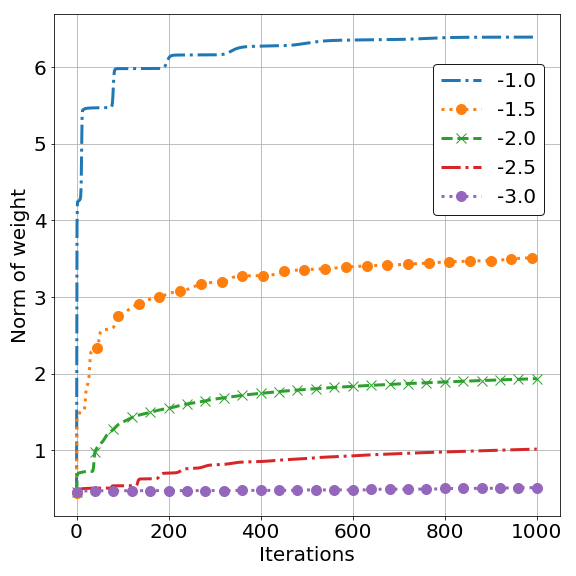
\includegraphics[width=0.5\textwidth]{figures/WN_direction.png}
\caption{Norm of parameters with different learning rate.}
\label{fig:weightnormgrowingnorm}
\end{figure}
}

\Answer{
${}$%placeholder
}

\end{exercise}

\begin{exercise}[5-5-5]
% (meta)
% Exercise contributed by chinwei
% label: ch10

\Exercise{
\label{ex:rnn_spectral}
This question is about activation functions and vanishing/exploding gradients in recurrent neural networks (RNNs). Let $\sigma:\R\rightarrow\R$ be an activation function. 
When the argument is a vector, we apply $\sigma$ element-wise. 
Consider the following recurrent unit:
$$\vh_t = \mW \sigma(\vh_{t-1}) + \mU\vx_t + \vb$$
\begin{enumerate}
\item Show that applying the activation function in this way is equivalent to the conventional way of applying the activation function: $\vg_t = \sigma(\mW\vg_{t-1} + \mU\vx_t + \vb)$ (i.e. express $\vg_t$ in terms of $\vh_t$).
\staritem Let $||\mA||$ denote the $L_2$ operator norm
\footnote{
The $L_2$ operator norm of a matrix $\mA$ is is an \textit{induced norm} corresponding to the $L_2$ norm of vectors. 
You can try to prove the given properties as an exercise.
}
of matrix $\mA$ ($||\mA||:=\max_{\vx:||\vx||=1}||\mA\vx||$). 
Assume $\sigma(x)$ has bounded derivative, i.e. $|\sigma'(x)|\leq \gamma$ for some $\gamma>0$ and for all $x$. We denote as $\lambda_1(\cdot)$ the largest eigenvalue of a symmetric matrix. Show that if the largest eigenvalue of the weights is upper-bounded by $\frac{\delta^2}{\gamma^2}$ for some $0 \leq \delta < 1$, gradients of the hidden state will vanish over time,    
 i.e.  
$$\lambda_1(\mW^\top\mW)\leq\frac{\delta^2}{\gamma^2} \quad\implies\quad \bigg{|}\bigg{|}\frac{\partial\vh_T}{\partial\vh_0}\bigg{|}\bigg{|}  \rightarrow0 \,\text{ as }\,T\rightarrow\infty$$

Use the following properties of the $L_2$ operator norm 
$$||\mA\mB||\leq||\mA||\,||\mB|| \qquad \text{ and } \qquad ||\mA||=\sqrt{\lambda_1(\mA^\top\mA)}$$

\item What do you think will happen to the gradients of the hidden state if the condition in the previous question is reversed, i.e. if the largest eigenvalue of the weights is larger than $\frac{\delta^2}{\gamma^2}$? 
Is this condition \textit{necessary} or \textit{sufficient} for the gradient to explode? (Answer in 1-2 sentences).
\end{enumerate}
}

\Answer{
${}$%placeholder
}


\end{exercise}

\begin{exercise}[6-12]
% (meta)
% Exercise contributed by Gabriele Prato
% label: ch10 

\Exercise{
\label{ex:bi_rnn_gradient}
Denote by $\sigma$ the logistic sigmoid function.
Consider the following Bidirectional RNN:
\begin{align*}
\vh^{(f)}_t & = \sigma(\mW^{(f)} \vx_t + \mU^{(f)} \vh^{(f)}_{t-1})\\
\vh^{(b)}_t & = \sigma(\mW^{(b)} \vx_t + \mU^{(b)} 
\vh^{(b)}_{t+1})\\
\vy_t & = \mV^{(f)} \vh^{(f)}_t + \mV^{(b)} \vh^{(b)}_t
\end{align*}
where the superscripts $f$ and $b$ correspond to the forward and backward RNNs respectively. 
\begin{enumerate}
\item Draw the computational graph for this RNN, unrolled for 3 time steps (from $t=1$ to $t=3$) Include and label the initial hidden states for both the forward and backward RNNs, $h_{0}^{(f)}$ and $h_{4}^{(b)}$ respectively. You may draw this by hand; you may also use a computer rendering package such as TikZ, but you are not required to do so.
Label each node and edge with the corresponding hidden unit or weight. 
\staritem Let $\vz_t$ be the true target of the prediction $\vy_t$ and consider the sum of squared loss $L=\sum_t L_t$ where $L_t=||\vz_t - \vy_t||_2^2$. 
Express the gradients $\nabla_{\vh_{t}^{(f)}}L$ and $\nabla_{\vh_{t}^{(b)}}L$ recursively
(in terms of $\nabla_{\vh_{t+1}^{(f)}}L$ and $\nabla_{\vh_{t-1}^{(b)}}L$ respectively).
Then derive $\nabla_{\mW^{(f)}}L$ and $\nabla_{\mU^{(b)}}L$.

\end{enumerate}
}

\Answer{
${}$%placeholder
}

\end{exercise}





\end{document}






\end{document}